\documentclass[11pt]{article}
\usepackage{graphicx}
\usepackage{rotating}
\usepackage{longtable}
\usepackage{lscape}
\usepackage{array}
\newcolumntype{L}[1]{>{\raggedright\let\newline\\\arraybackslash\hspace{0pt}}m{#1}}
\newcolumntype{C}[1]{>{\centering\let\newline\\\arraybackslash\hspace{0pt}}m{#1}}
\newcolumntype{R}[1]{>{\raggedleft\let\newline\\\arraybackslash\hspace{0pt}}m{#1}}
\usepackage{multirow}

\pagestyle{empty}

\newcommand{\bnot}[1]{\overline{{#1}}}
\newcommand{\band}{\cdot}
\newcommand{\bor}{+}
\newcommand{\set}{$\leftarrow$}
\newcommand{\rot}[1]{\begin{sideways}{\bf {#1}}\end{sideways}}
\newcommand{\blank}{\ \ \ \ \ }

% set page size

\setlength{\textwidth}{6.25truein}
\setlength{\textheight}{8.5truein}

% to center on sheet
\hoffset=-.8truein
\voffset -.5in
\parindent 0pt
\parskip 6pt

\newcommand{\HRule}{\rule{\linewidth}{0.3mm}}

\begin{document}

\vspace*{-1.1in}
\begin{center}
\HRule \\
\vspace{0.04in}
cs281: Computer Systems\\
\vspace{0.03in}
\Large{CPUlab -- ALU and Datapath}
\normalsize
\vspace*{-0.04in}
\HRule \\
\vspace{.05in}
Assigned: Oct.~30, Due: Nov.~8 at 11:59 pm\\
\rule{2.75in}{0.01in}

\end{center}

The objective of this exercise is twofold -- to complete a combinational circuit for an ALU that we can use with our Y86 CPU implementation, and to familiarize you with the Datapath of the Y86 CPU and to understand how, by manipulating control wires in the datapath, you can realize the semantic steps for the execution of each instructions' stages, from Fetch through Write-back and PC Update.

\subsection*{ALU Implementation}
You are being provided with a Logisim circuit file, \texttt{alulibrary.circ}.  This circuit file contains 32 bit versions of the functional units for the operations of add, and, xor, shift left, and shift right, as well as 32 bit versions of a 2-1 mux and a 4-1 mux.  Correct and complete implementations of \texttt{Add32}, \texttt{And32}, \texttt{Xor32}, \texttt{2-1Mux32}, and \texttt{4-1Mux32} have already been completed for you.  So your only task in \texttt{alulibrary.circ} is to provide implementations of \texttt{ShiftR32} and \texttt{ShiftL32}.  Both of these circuits have a 32 bit input (named \texttt{A32}) and a single bit input named \texttt{Cin}.  Both have a 32 bit output named \texttt{F32} and a single bit output named \texttt{Cout}.  These shifters always shift by exactly one bit, and use \texttt{Cin} for the value to shift ``in'' to the vacated bit. \texttt{F32} is the result, and the bit that would otherwise be shifted ``off'' and lost is given as \texttt{Cout}.

\begin{center}
\begin{tabular}{|l|l|}
\hline
Function & Semantics \\
\hline \hline
ShiftR32 & $F32 = A32$ \verb+>>+ 1; $F32_{31} = Cin$; $Cout = A32_0$ \\ \hline
ShiftL32 & $F32 = A32$ \verb+<<+ 1; $F32_{0} = Cin$; $Cout = A32_{31}$ \\
\hline
\end{tabular}
\end{center}

You are also being provided with a Logisim circuit file, \texttt{ALU.circ}.  In its \texttt{main} circuit, this circuit file contains a top level interface that will allow you to drive the \texttt{ALU32} circuit.  The \texttt{ALU32} circuit is where you will be doing your work, to implement the ALU as specified below, and using the \texttt{alulibrary} components completed in the first step.
\begin{center}
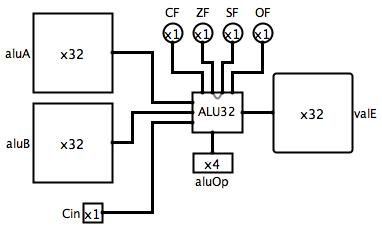
\includegraphics[scale=0.7]{y86_alutop}
\end{center}
The inputs are shown on the left and bottom of the ALU32 circuit and the outputs are on the right and top of the circuit.  The top of the chip is used for a set of single-bit outputs that comprise the condition code flags of ALU32.  Note that $aluA$ and $aluB$ are 32-bit-wide inputs, $aluOp$ is a 4-bit-wide input, and $Cin$ is a 1-bit-wide input.  $valE$ is an 32-bit-wide output, and $CF$, $ZF$, $SF$, and $OF$ are single bit outputs.

The $aluOp$ determines a particular operation for the combinational logic of the ALU32.  So, in general, we can think of the functionality as follows:
\[
(valE, CF, ZF, SF, OF) = aluOp(aluA, aluB, Cin)
\]
So the set of five outputs are a function, determined by $aluOp$, of the three inputs, $aluA$, $aluB$, and $Cin$.

$aluOp$ is a four bit-wide input, so in the table below, we give the bit pattern for $aluOp$, a mneumonic for the operation, and then the computation specifying the $valE$ output in terms of $aluA$, $aluB$, and $Cin$.  Since we all know C/C++ bitwise operations now, we will borrow that notation.
\small
\begin{center}
\begin{tabular}{|l|l|p{3in}|}
\hline
\bf{aluOp} & \bf{Mneumonic} & \bf{Semantics} \\ \hline \hline
0000 & add     &  	\texttt{valE = aluA + aluB}\\ \hline
0001 & sub & 	\verb|valE = aluA - aluB|\\ \hline
0010 & and &	\verb|valE = aluA & aluB|\\ \hline
0011 &xor&	 \verb|valE = aluA ^ aluB|\\ \hline
0100 & shiftR & \verb|valE = aluA >> 1;| valE$_{31} = Cin$ \\ \hline
0101 & shiftL & \verb|valE = aluA << 1;| valE$_0 = Cin$ \\ \hline
\end{tabular}
\end{center}
\normalsize

The following table gives the meanings for the four single bit condition codes.
\small
\begin{center}
\begin{tabular}{|c|C{.4in}|L{4.5in}|}
\hline
\bf{Flag} & \bf{Ops} & \bf{Description} \\ \hline \hline
ZF & {\em all}  & Zero Flag: If the result of the current ALU operation, $valE$, is zero, then $ZF$ is 1.  If the result of the operation is not zero, then $ZF$ is 0. \\ \hline \hline
SF & {\em all}  & Sign Flag:  Reflects the most significant bit of the result of the current ALU operation (i.e. valE$_{31}$).  When interpreted as an 32-bit two's complement, the sign bit indicates a negative result.\\ \hline \hline
\multirow{2}{*}{OF} & \texttt{add} \texttt{sub} & Overflow Flag: This bit is asserted if the current operation caused a two's complement overflow--either positive or negative, and is deasserted otherwise.  \\ \hline
 & \texttt{and\ \ } \texttt{\ \ \ xor\ \ \ }
\texttt{shiftR} \texttt{shiftL} & The $OF$ flag is 0 for all four of these other operations.  \\ \hline \hline
\multirow{2}{*}{CF}  &  \texttt{add} \texttt{sub} & Carry Flag: This bit is 1 if the addition caused a carry-out from the most significant bit position, so an unsigned overflow.  \\ \hline
& \texttt{shiftR} & This is the bit ``shifted off'' from operand $aluA$, aka aluA$_0$. \\ \hline
& \texttt{shiftL} & This is the bit ``shifted off'' from operand $aluA$, aka aluA$_{31}$. \\ \hline
& \texttt{and\ \ } \texttt{xor\ \ } & Always 0 for these two operations.\\ \hline
\end{tabular}
\end{center}
\normalsize

\noindent{\bf Restrictions and Advice}
\begin{itemize}
\item For digital logic components comprising aggregated 32 bit operations, you should use the implementations in the \texttt{alulibrary}.
\item You should not create a new component for subtract.  Find a way to use addition, and the best solutions will not use unnecessary digital logic.
\item You may, however, use the built-in Logisim multibit wide NOT gate.
\item Carefully follow the specification for the condition codes.  The ALU32 will be tested by a driver circuit that will check for correctness of {\em all} condition codes against all the different operations.
\end{itemize}

\subsection*{Datapath Familiarization}
Functional elements in the Datapath include:
\begin{description}
\item[PC]: Program Counter -- stateful device containing a 32 bit register holding the current program counter.  Input is the upcoming PC value, output is the current PC value.  A new program counter is stored on the rising clock edge.
\item[IMem]: Instruction Memory -- stateful device containing the Y86 program, starting at address 0.  Input is the 32 bit Program Counter, and output are the 6 consecutive bytes from memory starting at the PC address.  Internally, memory is loaded into four separate banks, each of which is 2 bytes wide, and loading must occur prior to instruction execution.  From that point on, the memory may be thought of as combinational, where, based on the PC as input, a six byte output is produced.
\item[ISplit]: Instruction Split -- combinational circuit whose inputs are the 6 (potential) bytes of the instruction and whose outputs are the union of the fields that make up all the Y86 instructions, including icode, ifun, rA, rB, Dest, and V/D.
\item[Registers]: Register File -- stateful device containing the eight Y86 registers, numbered from 0 to 7.  The register file is capable of routing to output the current values of {\em two} of its registers, as well as updating one or two registers.  Inputs are srcA and srcB, to determine values sent to the valA and valB outputs, as well as dstE/valE and dstM/valM, which determine register (and its associated value) to write on the next rising clock.  If dstE and/or dstM have value 0xF, then no register is updated.  Outputs valA and valB always reflect the current value of registers srcA and srcB.  
\item[ALU]: Arithmetic Logic Unit -- combinational circuit capable of performing addl, subl, andl, and xorl.  Inputs are ALUfun, ALU\_A, and ALU\_B.  Outputs are ZF, SF, OF, and valE. This currently loads \texttt{ALU32} from \texttt{ALU.circ}.
\item[CC]: Condition Codes -- stateful device implemented as a register holding the 3 1-bit values corresponding to ZF, SF, and OF.  In addition to these inputs, the register has an enable bit and an asynchronous reset bit as inputs.  The output is the current values of the three bits.  Updates occur on a rising clock if the enable is also asserted.
\item[DAddr]: Data Memory Address -- combinational circuit that, given a 32 bit aligned byte address yields a 20 bit word address suitable for input to the data memory.  The device also has a single bit indicating whether or not an illegal address was given as its input.
\item[DMem]: Data Memory -- stateful device used for the read/write data memory involved in a Y86 program.  Input is the 20 bit word address A to be read or written along with the 32 bit data value, D, to be modified as a result of a write.  Inputs also include a ``Store'' bit which, when 1, will cause the D value to be stored on the next rising clock edge, as well as an asynchronous reset for the memory.  Output is the 32-bit valM corresponding to the value in memory at the word address given by A.
\end{description}
In addition to these functional elements, the datapath consists of a set of multiplexers, one adder unit, and the set of wires connecting all of the elements.  The datapath can be made to ``execute'' instructions by manipulating the control bits, which in this initial datapath are simply input pins.  By setting all of these control inputs to particular values based on the current instruction and on other outputs of the functional elements (like the condition codes), we can manipulate the datapath into performing the semantics of our given instructions.

The Table below gives the meanings for each of the control signals on the Y86 datapath.

\begin{center}
\begin{longtable}{|c|c|p{4.5in}|}
\hline
\bf{Control} & \bf{Width} & \bf{Description} \\ \hline \hline
PCIncSrc & 2 & Determines value to add to PC to get to next instruction. \hspace{1in} 00 - 1, 01 - 2, 10 - 5, 11 - 6.\\ \hline
valCsrc & 1 & Determine value for valC. 0 means valC \set Dest (M4[PC+1]), 1 means valC \set V/D (M4[PC+2]). \\ \hline
valAsrc & 1 & Determine read register file output for valA. 0 means valA \set R[rA], 1 means valA \set R[\%esp].\\ \hline
valBsrc & 1 & Determine read register file output for valB. 0 means valB \set R[rB], 1 means valB \set R[\%esp]. \\ \hline
aluAsrc & 1 & Determine value to send to ALU\_A. 0 means ALU\_A \set valB, 1 means ALU\_A \set 0. \\ \hline
aluBsrc & 2 & Determine value to send to ALU\_B. 00 means ALU\_B \set valA, 01 means ALU\_B \set valC, 10 means ALU\_B \set 4, 11 means ALU\_B \set -4.\\ \hline
setCC & 1 & Determine whether or not to update the CC register on the next clock. 0 indicates do not update, 1 indicates update. \\ \hline
aluOp & 1 & Determine operation to route to ALUfun. 0 means 0000 (add), 1 means use ifun. \\ \hline
dmemAddr & 2 & Determine address routed to data memory address line. 00 means dAddr \set valE. 01 means dAddr \set valA. 10 and 11 mean to send address 0.\\ \hline
dmemData & 1 & Determine value routed to data memory D input. 0 means D \set valA, 1 means D \set valP \\ \hline
dmemWrite & 1 & Determine whether or not to store D at M4[dAddr] on the next clock. 0 indicates do not write memory, 1 indicates write memory. \\ \hline
dstEsrc & 2 & Determine destination register for write of valE. 00 means R[rB] \set valE, 01 means R[\%esp] \set valE, 10 and 11 mean send 0xf to dstE, indicating no write. \\ \hline
dstMsrc & 1 & Determine destination register for write of valM. 0 means R[rA] \set valM, 1 means send 0xf to dstM, indicating no write. \\ \hline
newPC & 2 & Determine source of next Program Counter to be routed to input of PC register. 00 means newPC \set valP, 01 means newPC \set valC, 10 means newPC \set valM, and 11 is undefined. \\ \hline
\end{longtable}
\end{center}

\noindent{\bf Datapath Assignment}

Your task in this part of the assignment is twofold:
\begin{enumerate}
\item Learn the datapath by manually executing instructions in the datapath.  A few initial instructions are given in the files example.ys and example.yo and their associated Logisim instruction memory image exbank0.mem, exbank1.mem, exbank2.mem, and exbank3.mem.  Your professor will lead you through the first couple and general instructions are given below.
\item Your second task is to complete the table at the end of this handout completely defining the control functionality for all the given instructions.  Based on the semantics of the instructions, you should determine the correct control signals for that instruction.  The instruction semantics are given through the phases of the datapath in the textbook figures 4.18 through 4.21, and in the class handout.  You should use both pencil and paper as well as Logisim experimental techniques to determine these values.
\end{enumerate}

Steps to execute one or more instructions:
\begin{enumerate}
\item Begin at the Datapath circuit on the canvas with the pointer tool selected. Open \texttt{Y86.circ} and double-click the Datapath circuit in the explorer pane to make it the active circuit if this is not the case.
\item Right-click on the IMem device and select the `View Memory' option.  The four memory banks that you see there are ROMs and are preloaded with the instruction memory corresponding to the file(s) \texttt{example.ys}/texttt{example.yo}.  If you wish to load instruction memory with a different program, do the following:
\begin{itemize}
\item For each of the memory banks, from top to bottom, you should right-click on the memory device and select the `Load Image...' option.
\item Navigate in the file system and select the memory image appropriate to the particular bank (0, 1, 2, or 3).
\end{itemize}
\item Double-click on the Datapath circuit again to make it the active circuit.
\item Select the `hand' tool so that we can manipulate values on the Datapath.
\item Take the clock to an asserted level.
\item Assert and then deassert the Reset pin.  At this point, the PC, CC, and registers are initialized to zero and you should be able to see the values derivative of the first instruction at the probe displays (like icode, ifun, rA, and rB).
\item \label{cyclestart} Instruction execution occurs in a single clock cycle.  Once the instruction is available from IMem following the rising edge of the clock, we need to, based on the particular instruction, set the pins associated with the control signals in the datapath.  Eventually, this manual operation will be replaced by a combinational circuit that performs the same task.  For now, with the clock still high, set the control signals PCIncSrc, valCsrc, valAsrc, valBsrc, aluAsrc, aluBsrc, setCC, aluOp, dmemAddr, dmemData, dmemWrite, dstEsrc, dstMsrc, and newPC to the correct values {\em based on the instruction being executed}.  The professor will take you through the example of irmovl.  

For irmovl, the values to be set include PCIncSrc=11, valCsrc=1, aluAsrc=1, aluBsrc=01, setCC=0, aluOp=0, dmemAddr=10, dmemWrite=0, dstEsrc=00, dstMsrc=1and newPC=00.  

% if set correctly, valP = 6, valC = 5, valA and valB Don't Care, valE=5, dAddr=0, valM Don't Care, dstE=0, dstM=f

%For addl, the values to be set include PCIncSrc=01, valAsrc=0, valBsrc=0, dstEsrc=00, dstMsrc=1, aluAsrc=00, aluBsrc=0, setCC=1, aluOp=1, dmemWrite=0, and newPC=00.

\item Once the control signals have been set, check the values from left to right through the datapath.  Based on the register transfer semantics of the various instructions given in Tables 4.18 through 4.21 in your book, do the values of valP, valC, valA, valB, etc. correspond to the specific instruction being executed?  If they do not, then verify your control signals again.
\item When the values/control signals are correct, change the clock to come down to the deasserted state.  Note that when the clock goes low, the negation in the lower left of the datapath will cause the clock input to the register file, the CC register, the data memory, and the PChold register to go high.  So by bringing the clock low, these devices will take any write-values on their input and store them into their device.  This, in effect, ``seals the deal'' for the execution of this instruction and we are ready to go on to the next instruction.
\item Change the clock back to the high/asserted state.  The value of newPC is now stored in PC and we go back to step~\ref{cyclestart} and set the control signals appropriately.
\end{enumerate}

When filling out the table below, if the value for a given entry is dependent on some other state in the datapath, use a footnote and explain the conditions under which the entry would have one value or another.  Also, for full credit, you should employ "Don't Care" values of X where appropriate.
\begin{center}
\begin{tabular}{|l|r|r|r|r|r|r|r|r|r|r|r|r|r|r|}
\hline
{\bf Instruction} & \rot{PCIncSrc} & \rot{valCsrc} & \rot{valAsrc} & \rot{valBsrc}  & \rot{aluAsrc} & \rot{aluBsrc} & \rot{setCC} & \rot{aluOp} & \rot{dmemAddr} & \rot{dmemData} & \rot{dmemWrite\ } & \rot{dstEsrc} & \rot{dstMsrc} & \rot{newPC} \\
\hline \hline
& & & & & & & & & & & & & & \\
halt & \blank & \blank & \blank & \blank & \blank & \blank & \blank & \blank & \blank & \blank & \blank & \blank & \blank & \blank  \\
\hline
& & & & & & & & & & & & & & \\
nop & \blank & \blank & \blank & \blank & \blank & \blank & \blank & \blank & \blank & \blank & \blank & \blank & \blank & \blank  \\
\hline
& & & & & & & & & & & & & & \\
rrmovl rA,rB & \blank & \blank & \blank & \blank & \blank & \blank & \blank & \blank & \blank & \blank & \blank & \blank & \blank & \blank  \\
\hline
& & & & & & & & & & & & & & \\
irmovl V,rB & \blank & \blank & \blank & \blank & \blank & \blank & \blank & \blank & \blank & \blank & \blank & \blank & \blank & \blank  \\
\hline
& & & & & & & & & & & & & & \\
rmmovl rA,D(rB) & \blank & \blank & \blank & \blank & \blank & \blank & \blank & \blank & \blank & \blank & \blank & \blank & \blank & \blank  \\
\hline
& & & & & & & & & & & & & & \\
mrmovl D(rB),rA & \blank & \blank & \blank & \blank & \blank & \blank & \blank & \blank & \blank & \blank & \blank & \blank & \blank & \blank  \\
\hline
& & & & & & & & & & & & & & \\
OPl rA,rB & \blank & \blank & \blank & \blank & \blank & \blank & \blank & \blank & \blank & \blank & \blank & \blank & \blank & \blank  \\
\hline
& & & & & & & & & & & & & & \\
jXX Dest & \blank & \blank & \blank & \blank & \blank & \blank & \blank & \blank & \blank & \blank & \blank & \blank & \blank & \blank  \\
\hline
& & & & & & & & & & & & & & \\
cmovXX rA, rB & \blank & \blank & \blank & \blank & \blank & \blank & \blank & \blank & \blank & \blank & \blank & \blank & \blank & \blank  \\
\hline
& & & & & & & & & & & & & & \\
call Dest & \blank & \blank & \blank & \blank & \blank & \blank & \blank & \blank & \blank & \blank & \blank & \blank & \blank & \blank  \\
\hline
& & & & & & & & & & & & & & \\
ret & \blank & \blank & \blank & \blank & \blank & \blank & \blank & \blank & \blank & \blank & \blank & \blank & \blank & \blank  \\
\hline
& & & & & & & & & & & & & & \\
pushl rA & \blank & \blank & \blank & \blank & \blank & \blank & \blank & \blank & \blank & \blank & \blank & \blank & \blank & \blank  \\
\hline
& & & & & & & & & & & & & & \\
popl rA & \blank & \blank & \blank & \blank & \blank & \blank & \blank & \blank & \blank & \blank & \blank & \blank & \blank & \blank  \\
\hline
\end{tabular}
\end{center}

\end{document}


 

 